% ******************************* PhD Thesis Template **************************
% Please have a look at the README.md file for info on how to use the template


% \documentclass[a4paper,12pt,times,numbered,print,index,oneside]{Classes/PhDThesisPSnPDF}

%\documentclass[a4paper,12pt,Boisik,numbered,print,index,oneside]{Classes/PhDThesisPSnPDF}

\documentclass[a4paper,12pt,Palatino,numbered,print,index,oneside]{Classes/PhDThesisPSnPDF}

\usepackage{listings}
\usepackage{color}
\usepackage{shapepar}
\usepackage[T1]{fontenc}
\usepackage[utf8]{inputenc}
\usepackage{hyperref}

\definecolor{dkgreen}{rgb}{0,0.6,0}
\definecolor{gray}{rgb}{0.5,0.5,0.5}
\definecolor{mauve}{rgb}{0.58,0,0.82}
\definecolor{light-gray}{gray}{0.70}

\lstset{
%frame=none,
frame=single,
language=Python,
aboveskip=3mm,
belowskip=3mm,
showstringspaces=false,
columns=flexible,
basicstyle={\small\ttfamily},
numbers=none,
numberstyle=\tiny\color{gray},
keywordstyle=\color{blue},
commentstyle=\color{dkgreen},
stringstyle=\color{mauve},
breaklines=true,
breakatwhitespace=true,
tabsize=3
}

\usepackage{color}
\usepackage{xcolor}

\usepackage{amsmath}
\usepackage{algorithm}

\usepackage[noend]{algpseudocode}
\algdef{SE}{Begin}{End}{\textbf{begin}}{\textbf{end}}

\usepackage{caption}

\usepackage{subfig}

\DeclareCaptionFont{white}{\color{white}}
\DeclareCaptionFormat{listing}{\colorbox{black}{\parbox{\textwidth}{#1#2#3}}}
\captionsetup[lstlisting]{format=listing,labelfont=white,textfont=white, margin=0pt}

% \usepackage{titlesec}
% \newcommand*{\justifyheading}{\raggedleft}
% \titleformat{\chapter}[display]
%   {\normalfont\huge\bfseries\justifyheading}{\chaptertitlename\ \thechapter}
%   {20pt}{\Huge}

% \usepackage{indentfirst}

% ******************************************************************************
% ******************************* Class Options ********************************
% *********************** See README for more details **************************
% ******************************************************************************

% `a4paper'(The University of Cambridge PhD thesis guidelines recommends a page
% size a4 - default option) or `a5paper': A5 Paper size is also allowed as per
% the Cambridge University Engineering Deparment guidelines for PhD thesis
%
% `11pt' or `12pt'(default): Font Size 10pt is NOT recommended by the University
% guidelines
%
% `oneside' or `twoside'(default): Printing double side (twoside) or single
% side.
%
% `print': Use `print' for print version with appropriate margins and page
% layout. Leaving the options field blank will activate Online version.
%
% `index': For index at the end of the thesis
%
% `draftclassic': For draft mode without loading any images (same as draft in book)
%
% `draft': Special draft mode with line numbers, images, and water mark with
% timestamp and custom text. Position of the text can also be modified.
%
% `abstract': To generate only the title page and abstract page with
% dissertation title and name, to submit to the Student Registry
%
% `chapter`: This option enables only the specified chapter and it's references
%  Useful for review and corrections.
%
% ************************* Custom Page Margins ********************************
%
% `custommargin`: Use `custommargin' in options to activate custom page margins,
% which can be defined in the preamble.tex. Custom margin will override
% print/online margin setup.
%
% *********************** Choosing the Fonts in Class Options ******************
%
% `times' : Times font with math support. (The Cambridge University guidelines
% recommend using times)
%
% `fourier': Utopia Font with Fourier Math font (Font has to be installed)
%            It's a free font.
%
% `customfont': Use `customfont' option in the document class and load the
% package in the preamble.tex
%
% default or leave empty: `Latin Modern' font will be loaded.
%
% ********************** Choosing the Bibliography style ***********************
%
% `authoryear': For author-year citation eg., Krishna (2013)
%
% `numbered': (Default Option) For numbered and sorted citation e.g., [1,5,2]
%
% `custombib': Define your own bibliography style in the `preamble.tex' file.
%              `\RequirePackage[square, sort, numbers, authoryear]{natbib}'.
%              This can be also used to load biblatex instead of natbib
%              (See Preamble)
%
% **************************** Choosing the Page Style *************************
%
% `default (leave empty)': For Page Numbers in Header (Left Even, Right Odd) and
% Chapter Name in Header (Right Even) and Section Name (Left Odd). Blank Footer.
%
% `PageStyleI': Chapter Name next & Page Number on Even Side (Left Even).
% Section Name & Page Number in Header on Odd Side (Right Odd). Footer is empty.
%
% `PageStyleII': Chapter Name on Even Side (Left Even) in Header. Section Number
% and Section Name in Header on Odd Side (Right Odd). Page numbering in footer

% Uncomment to change page style
%\pagestyle{PageStyleII}

% ********************************** Preamble **********************************
% Preamble: Contains packages and user-defined commands and settings
% ******************************************************************************
% ****************************** Custom Margin *********************************
\usepackage[italian,english]{babel}

% Add `custommargin' in the document class options to use this section
% Set {innerside margin / outerside margin / topmargin / bottom margin}  and
% other page dimensions
\ifsetCustomMargin
  \RequirePackage[left=37mm,right=30mm,top=35mm,bottom=30mm]{geometry}
  \setFancyHdr % To apply fancy header after geometry package is loaded
\fi

% Add spaces between paragraphs
%\setlength{\parskip}{0.5em}
% Ragged bottom avoids extra whitespaces between paragraphs
\raggedbottom
% To remove the excess top spacing for enumeration, list and description
%\usepackage{enumitem}
%\setlist[enumerate,itemize,description]{topsep=0em}

% *****************************************************************************
% ******************* Fonts (like different typewriter fonts etc.)*************

% Add `customfont' in the document class option to use this section

\ifsetCustomFont
  % Set your custom font here and use `customfont' in options. Leave empty to
  % load computer modern font (default LaTeX font).
  %\RequirePackage{helvet}

  % For use with XeLaTeX
  %  \setmainfont[
  %    Path              = ./libertine/opentype/,
  %    Extension         = .otf,
  %    UprightFont = LinLibertine_R,
  %    BoldFont = LinLibertine_RZ, % Linux Libertine O Regular Semibold
  %    ItalicFont = LinLibertine_RI,
  %    BoldItalicFont = LinLibertine_RZI, % Linux Libertine O Regular Semibold Italic
  %  ]
  %  {libertine}
  %  % load font from system font
  %  \newfontfamily\libertinesystemfont{Linux Libertine O}
\fi

% *****************************************************************************
% **************************** Custom Packages ********************************

% ************************* Algorithms and Pseudocode **************************

%\usepackage{algpseudocode}


% ********************Captions and Hyperreferencing / URL **********************

% Captions: This makes captions of figures use a boldfaced small font.
%\RequirePackage[small,bf]{caption}

\RequirePackage[labelsep=space,tableposition=top]{caption}
\renewcommand{\figurename}{Fig.} %to support older versions of captions.sty


% *************************** Graphics and figures *****************************

%\usepackage{rotating}
%\usepackage{wrapfig}

% Uncomment the following two lines to force Latex to place the figure.
% Use [H] when including graphics. Note 'H' instead of 'h'
%\usepackage{float}
%\restylefloat{figure}

% Subcaption package is also available in the sty folder you can use that by
% uncommenting the following line
% This is for people stuck with older versions of texlive
%\usepackage{sty/caption/subcaption}
% \usepackage{subcaption}

% ********************************** Tables ************************************
\usepackage{booktabs} % For professional looking tables
\usepackage{multirow}

%\usepackage{multicol}
%\usepackage{longtable}
%\usepackage{tabularx}


% *********************************** SI Units *********************************
\usepackage{siunitx} % use this package module for SI units


% ******************************* Line Spacing *********************************

% Choose linespacing as appropriate. Default is one-half line spacing as per the
% University guidelines

% \doublespacing
\onehalfspacing
% \singlespacing


% ************************ Formatting / Footnote *******************************

% Don't break enumeration (etc.) across pages in an ugly manner (default 10000)
%\clubpenalty=500
%\widowpenalty=500

%\usepackage[perpage]{footmisc} %Range of footnote options


% *****************************************************************************
% *************************** Bibliography  and References ********************

%\usepackage{cleveref} %Referencing without need to explicitly state fig /table

% Add `custombib' in the document class option to use this section
\ifuseCustomBib
   \RequirePackage[square, sort, numbers, authoryear]{natbib} % CustomBib

% If you would like to use biblatex for your reference management, as opposed to the default `natbibpackage` pass the option `custombib` in the document class. Comment out the previous line to make sure you don't load the natbib package. Uncomment the following lines and specify the location of references.bib file

% \RequirePackage[backend=biber, style=numeric-comp, citestyle=numeric, sorting=nty, natbib=true]{biblatex}
% \bibliography{References/references} %Location of references.bib only for biblatex

\fi

% changes the default name `Bibliography` -> `References'
\renewcommand{\bibname}{References}


% ******************************************************************************
% ************************* User Defined Commands ******************************
% ******************************************************************************

% *********** To change the name of Table of Contents / LOF and LOT ************

%\renewcommand{\contentsname}{My Table of Contents}
%\renewcommand{\listfigurename}{My List of Figures}
%\renewcommand{\listtablename}{My List of Tables}


% ********************** TOC depth and numbering depth *************************

\setcounter{secnumdepth}{2}
\setcounter{tocdepth}{2}


% ******************************* Nomenclature *********************************

% To change the name of the Nomenclature section, uncomment the following line

%\renewcommand{\nomname}{Symbols}


% ********************************* Appendix ***********************************

% The default value of both \appendixtocname and \appendixpagename is `Appendices'. These names can all be changed via:

%\renewcommand{\appendixtocname}{List of appendices}
%\renewcommand{\appendixname}{Appndx}

% *********************** Configure Draft Mode **********************************

% Uncomment to disable figures in `draft'
%\setkeys{Gin}{draft=true}  % set draft to false to enable figures in `draft'

% These options are active only during the draft mode
% Default text is "Draft"
%\SetDraftText{DRAFT}

% Default Watermark location is top. Location (top/bottom)
%\SetDraftWMPosition{bottom}

% Draft Version - default is v1.0
%\SetDraftVersion{v1.1}

% Draft Text grayscale value (should be between 0-black and 1-white)
% Default value is 0.75
%\SetDraftGrayScale{0.8}


% ******************************** Todo Notes **********************************
%% Uncomment the following lines to have todonotes.

%\ifsetDraft
%	\usepackage[colorinlistoftodos]{todonotes}
%	\newcommand{\mynote}[1]{\todo[author=kks32,size=\small,inline,color=green!40]{#1}}
%\else
%	\newcommand{\mynote}[1]{}
%	\newcommand{\listoftodos}{}
%\fi


% \titleformat{\chapter}[chapter]{\filleft\Huge\bfseries}{\thechapter\hsp\textcolor{gray75}{|}\hsp}{0pt}{\Huge\bfseries}

\begin{document}
\selectlanguage{italian}

% ************************ Thesis Information & Meta-data **********************
% Thesis title and author information, refernce file for biblatex
\begin{titlepage}
\begin{center}


{\large Università degli Studi di Salerno}\\[0.2truecm]
{\large Dipartimento di Informatica}\\

% \vfill

\begin{figure}[htbp]
\centering

\includegraphics[height=3cm, width=3cm]{Figure/logounisa.png}
\end{figure}

% \vfill

{\large Corso di Laurea in Informatica}

\vfill\vfill

{\Huge \textbf{TiveJS}}

\vspace{0.2cm}

{\LARGE Un'applicazione Javascript per il riconoscimento di linguaggi diagrammatici} 
\newline \newline
{\LARGE A Javascript application for the recognition of Diagrammatic languages}

\vfill\vfill

{\bf Relatori}              \hfill {\bf Candidato}  \\
Prof. Gennaro Costagliola   \hfill Dario Tecchia  \\
Dott. Mattia De Rosa        \hfill Matr. 0512102581 \\

\vfill
\hrulefill 

Anno Accademico 2018/2019

\end{center}
\end{titlepage}

% ***************************** Abstract Separate ******************************

\ifdefineAbstract
    \includeonly{Abstract/abstract}
\fi

% ******************************** Front Matter ********************************

\begin{dedication}

\begin{flushright}

\textit{Questa tesi la dedico alla mia famiglia.}

\end{flushright}

\end{dedication}

\newpage

\chapter*{Ringraziamenti}
\addcontentsline{toc}{chapter}{Ringraziamenti}

\newpage

\chapter*{Abstract}
\addcontentsline{toc}{chapter}{Abstract}

    La comunicazione visiva è in molti casi più diretta ed immediata rispetto alla comunicazione verbale: disegni, foto e mappe sono esempi di frasi visive che necessitano di un contesto per essere descritte in modo naturale.
    \newline
    In questa tesi presento TiveJS, un'estensione della piattaforma \href{https://www.draw.io/}{draw.io}, che sfrutta  simboli e  definizioni sematiche per il riconoscimento dei linguaggi diagrammatici e la traduzione di questi in altri linguaggi.
    Il tool applica  delle definizioni semantiche  ad un diagramma e restituisce una traduzione di quest'ultimo. La traduzione avviene attraverso due fasi principali: il riconoscimento del grafo e l'applicazione delle definizioni.
    \newline
    Il mio lavoro di tesi si basa su strumenti precedentemente sviluppati: LoCoModeler e Tive. Precedentemente suddiviso in lato client e lato server, Tive è stato re-implementato completamente in JavaScript, prendendo il nome di TiveJS, eliminando così la necessità del server.


% *********************** Adding Table of Contents ***********************

\tableofcontents

\newpage

\listoffigures

% ******************************** Main Matter *********************************

\mainmatter

\chapter{Introduzione}

    La comunicazione fra individui avviene in svariati modi, ad esempio attraverso il linguaggio verbale ed il linguaggio visivo (o linguaggio visuale).
    \newline
    Un linguaggio visuale non è altro che una forma di comunicazione, detta comunicazione visuale, che fa uso di simboli grafici o immagini. Simboli grafici, immagini e mappe sono esempi di elementi utilizzati all'interno della comunicazione visiva (o comunicazione visuale) che necessitano di un contesto per essere descritte in modo naturale. Spesso quest'ultima risulta essere molto più immediata e di facile comprensione rispetto alla tradizionale comunicazione verbale coposta di lettere e parole.
    \newline
    In questa tesi presento \textbf{TiveJS}, un'estensione della piattaforma \href{https://www.draw.io/}{draw.io}, che sfrutta  simboli e  definizioni sematiche per il riconoscimento dei linguaggi diagrammatici e la traduzione di questi in altri linguaggi.

    \section{Motivazioni}
        La piattaforma già esistente, LoCoMoTiVE, si basa su un meccanisco client-server.
        \newline
        Il client è formato dalla piattaforma draw.io, opportunamente modifica, per la creazione di sentenze visuali.
        Il server è stato implementato in Java utilizzando i servlet per il riconoscimento e la traduzione delle sentenze visuali.
        Il funzionamento è molto semplice, il client esegue una chiamata HTTP di tipo POST contenute al suo interno un grafo o un diagramma, creato attraverso l'utilizzo di simboli ad hoc, in formato XML.~Una volta ricevuta la sentenza visuale, il server la interpreta applicando le definizioni per poi restituire la traduzione semantica oppure dei messaggi di errore.
        \newline
        Le motivazioni che ci hannno portato alla creazione di un nuovo tool sono varie: rendere l'applicazione più scalabile e più veloce limitando l'interazione con il server a semplici accessi a pagine statiche; l'aggiornamento di TiVe all'ultima versione di draw.io.
        Essendo il core di TiveJS scritto completamente in JavaScript ora si integra perfettamente con la piattaforma estesa e con la manipolazione del grafo.
        Le definizioni dei linguaggi ora sono definite in formato JSON rendendo ancora più alta l'interoperabilità dei sistemi. 

    \section{Lavori Correlati}
        Il mio lavoro di tesi, essendo principalmente un porting ed una rivisitazione, si basa su strumenti precedentemente sviluppati.
        Gli strumenti in questione sono descritti nel dettaglio nei seguenti sottoparagrafi.

        \subsection{draw.io e mxGraph}

        \begin{figure}[htbp]
            \centering
            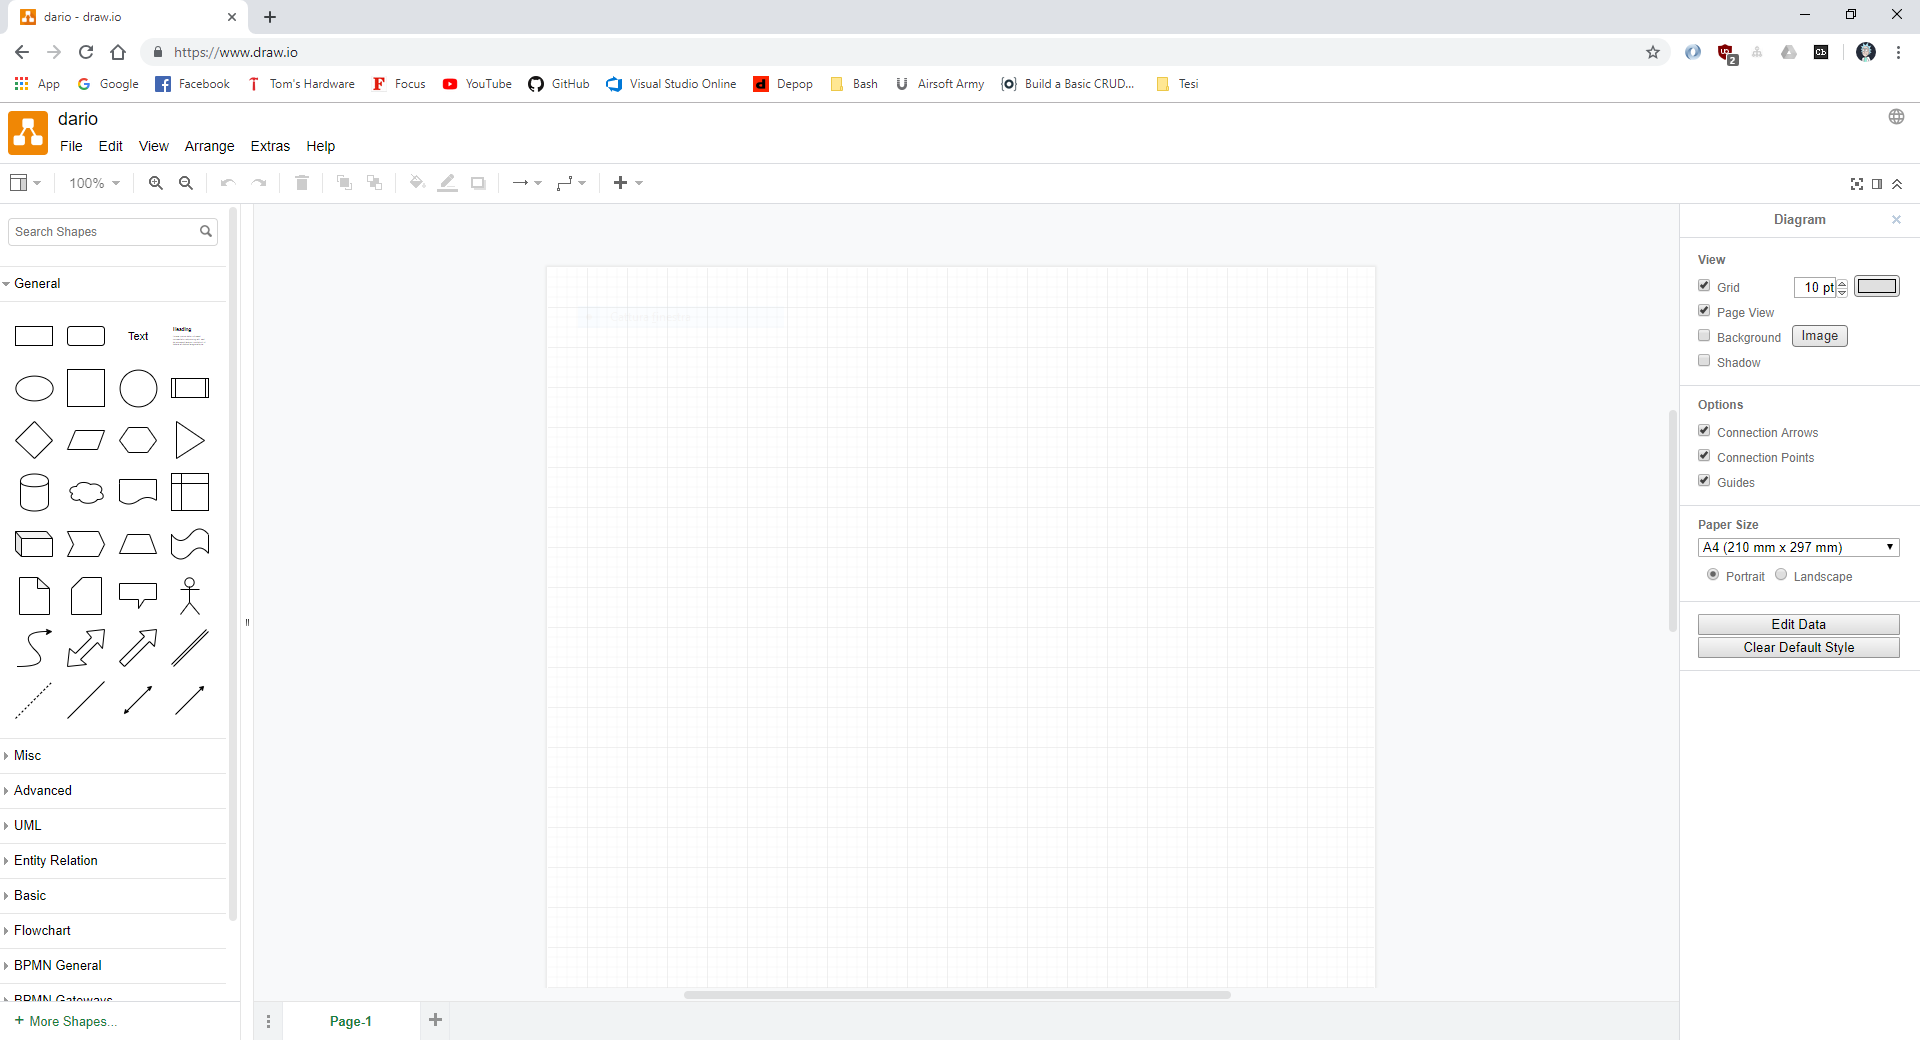
\includegraphics[scale=0.17]{Figure/drawio.png}
            \caption{Schermata di draw.io}
            \label{fig:drawio}
        \end{figure}

            TiveJS, è basato su draw.io, un'applicazione web gratis che permette agli utenti di creare diagrammi e grafi direttamente dal proprio browser web, mostrato in figura \ref{fig:drawio}. Ha un'integrazione con Google Drive e Dropbox per il salvataggio di dati che può avvenire anche con l'ausilio del localStorage del browser o attraverso il salvataggio di file sulla macchina. Draw.io è basato sulla libreria mxGraph.
            \newline
            Il software è stato sviluppato nel 2005 dalla JGraph Ltd.

        \subsection{LoCoMoTiVE}
            
            All'attuale stato dell'arte troviamo l'ecosistema LoCoMoTiVE, ovvero un'unione di due software, LoCoModeler e Tive. Presentato in~\cite{extending_localcontext} e~\cite{localcontext}, questo tool permette l'analisi semantica basata sul contesto locale, vista nel dettaglio nel capitolo~\ref{ch:chapter3}. Nei prossimi due paragrafi andrò ad illustrare singolarmente i due componenti di cui è composto.

            \newpage

            \subsubsection{LoCoModeler}
            
                \begin{figure}[htbp]
                    \centering
                    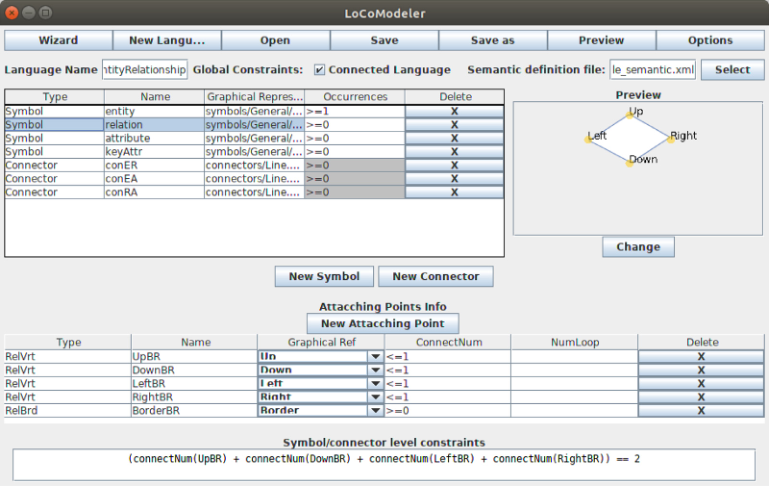
\includegraphics[scale=1.5]{Figure/locomodeler.png}
                    \caption{Schermata di LoCoModeler}
                    \label{fig:locomodeler}
                \end{figure}

                Come descritto in \cite{extending_localcontext}, il modulo LoCoModeler consente ai designer la creazione e la modifica del linguaggio visivo in base al contesto locale, in maniera rapida e facile. Il suo output è la definizione in formato XML del linguaggio che verrà utilizzato durante il riconoscimento dei diagrammi. Una volta che il progettista ha completato la specifica del linguaggio, può compilarlo in un ambiente web (il modulo TiVE) per consentire agli utenti di disegnare frasi e verificarne la correttezza. Durante la definizione del linguaggio, questa funzione consente al progettista di controllare la correttezza delle specifiche.
                \newline
                Una schermata principale dell'interfaccia grafica del tool è mostrata nella Figura \ref{fig:locomodeler}. Le sue componenti principali sono:
                \begin{itemize}
                    \item Una casella di testo contenente il nome del linguaggio e una checkbox che sta ad indicare se il diagramma o grafo deve essere o non essere necessariamente connesso\footnote{Un grafo è detto connesso se, per ogni coppia di vertici $(u, v)\in{V}$, esiste un cammino che collega u a v.}.
                    \item Una tabella riportante le informazioni principali dei simboli e dei connettori inclusi nel linguaggio. E' possibile modificare o eliminare un elemento interagendo con la riga di questo. L'utente può aggiungere nuovi simboli o connettori usando i bottoni sottostanti la tabella.
                    \item Un pannello (sulla destra) mostra un'anteprima grafica del simbolo o connettore selezionato nella tabella. E' possibile cambiare la rappresentazione grafica dell'elemento utilizzando il bottone \textit{Change}.
                    \item Una tabella (al centro) mostra le informazioni relative al simbolo o connettore selezionato. Ogni riga mostra un punto d'attacco e i relativi vincoli. E' possibile aggiungere nuove righe utilizzando i bottoni sovrastanti la tabella.
                    \item Un'area di testo dove è possibile specificare i vincoli per il simbolo o il connettore attraverso espressioni simili al C\footnote{Linguaggio di programmazione.}.
                \end{itemize}
                La definizione di un nuovo linguaggio può avvenire grazie all'ausilio di un \textit{Wizard} diviso in tre fasi.

            \subsubsection{TiVE}

                \begin{figure}[htbp]
                    \centering
                    \includegraphics[scale=0.7]{Figure/tive.png}
                    \caption{Schermata di TiVE}
                    \label{fig:tive}
                \end{figure}

                Una volta definito il linguaggio, i diagrammi possono essere composti utilizzando i simboli e i connettori definiti nella sua specifica. Questo può essere fatto attraverso un editor grafico TiVE, che è un'applicazione web che consente la composizione di diagrammi direttamente dal browser web.
                \newline
                Come mostrato nella Figura~\ref{fig:tive}, l'applicazione è costituita da tre sezioni principali:
                \begin{itemize}
                    \item Nella toolbar a sinistra troviamo la palette dei simboli e connettori utlizzabili per la creazione dei diagrammi.
                    \item Nella zona centrale troviamo l'area di lavoro dove è possibile comporre i diagrammi trascinando gli elementi contenuti nella toolbar di sinistra.
                    \item A destra troviamo la Console dove verrà mostrata la traduzione semantica o la lista di errori nel caso in cui si verificassero.
                \end{itemize}

    \section{Organizzazione della Tesi}
        Nel capitolo 2 tratterò dei linguaggi visuali e dei loro componenti fondamentali. Nel capitolo 3 parlerò del Local Context e delle corrsipondenti specifiche sintattiche e semantiche. Nel capitolo 4 introdurrò il risultato del mio lavoro di tesi, TiveJS e le sue funzioni, e illustrerò  i dettagli dell' implementazione e le tecnologie usate. Nel capitolo 5 illustrerò vari casi d'utilizzo da me studiati. Nel capitolo 6, presenterò le conclusioni e possibili sviluppi futuri dell'applicazione.

\chapter{Linguaggi visuali}

    Nei precedenti capitoli ho parlato spesso di linguaggi verbali e linguaggi visuali e di quanto la comunicazione visuale può essere più efficiente della comunicazione verbale. In questo capitolo entrerò nel dettaglio senza dilungarmi andando ad illustrare quali sono le principali differenze tra un linguaggio visuale ed uno verbale, i componenti che lo compongono e in quali casi o contesti un linguaggi visivo è più efficace rispetto ad uno verbale.

    \section{Linguaggio verbale}
    Il linguaggio verbale è un gruppo di elementi, come suoni e parole, che messe insieme formano frasi e infine permettono la comunicazione fra individui. Da questo deriva la comunicazione verbale che è quindi costitutita dalle parole usate quando parliamo o scriviamo.

    \section{Componenti}
    Ogni linguaggio è formato da un proprio insieme di componenti. Un linguaggio visuale si distingue principalmente dal linguaggio verbale per i componenti di cui è formato. Il linguaggio visivo si basa su simboli grafici o immagini. Elementi che il cervello umano interpreta e trasforma in concetti, linguaggio verbale ed emozioni. Quindi se il linguaggio visuale è costitutito da testo e parole per la formazioni di frasi, il linguaggio visivo è formato da simboli e disegni per formare sentenze visive.
    Una componente fondamentale di un linguaggio visuale è il contesto che viene dato ad ogni simboli appartenente ad una frase visiva.
    \newline
    \begin{figure}[htbp]
        \centering
        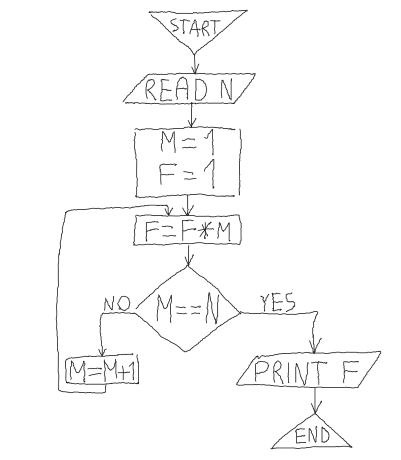
\includegraphics[scale=0.6]{Figure/diagram.PNG}
        \caption{Esempio di sentenza visiva, da~\cite{localcontext_recognition}}
        \label{fig:diagram}
    \end{figure}
    \newline
    Ad esempio, come possiamo notare avvalendoci del disegno in figura~\ref{fig:diagram}, senza un contesto sono semplici simboli connessi fra loro da delle frecce. Invece, dando una definizione ai simboli del diagramma può essere interpretato come un diagramma di flusso o \textit{Flowchart}\footnote{Il diagramma di flusso (o \textit{Flowchart}), in informatica, è una rappresentazione grafica delle operazioni da eseguire per l'esecuzione di un algoritmo.}.

    \section{Vantaggi}
    I vantaggi possono essere molteplici, innanzitutto un linguaggio visuale può essere molto più efficace e di facile comprensione rispetto al linguaggio verbale per via della sua semplicità e naturalità. Non ha lingue o convenzioni in quanto un disegno o un'immagina non dipende da lingue o standard.

\chapter{Local Context}\label{ch:chapter3}
    \section{Sintassi}
    \section{Semantica}

\chapter{TiveJS}
    \section{Funzionamento}
        \subsubsection{Riconoscimento grafo}
        \subsubsection{Applicazione definizioni}
    \section{Implementazione}
        \subsection{Tecnologie usate}

\chapter{Contesti d'utilizzo}
    \section{Entitiy Relationship}
    \section{Flowchart}
    \section{Tree}

\chapter{Conclusioni}

    \section{Sviluppi futuri}

% ********************************** Appendices ********************************

\begin{appendices} % Using appendices environment for more functionality

\chapter{Codici}
    \begin{spacing}{0.5}
        \lstinputlisting[language=JavaScript, caption={\textbf{Specifica di un linguaggio in formato XML, in questo caso quello per Albero Binario}}, label={appendix:xml_definition}, language=Xml]{SourceCode/tree_specific.xml}
        \newpage
        \lstinputlisting[language=JavaScript, basicstyle=\scriptsize, caption={\textbf{Specifica sintattica di un Albero}}, label={appendix:jsonDefinition}, language=Xml]{SourceCode/newDefinition.json}
        \newpage
        \lstinputlisting[language=JavaScript, caption={\textbf{Specifica semantica di un linguaggio in formato JSON, in questo caso quello per Albero}}, label={appendix:jsonSemanticDefinition}, language=Xml]{SourceCode/newSemanticDefinition.json}
    \end{spacing}
    \begin{spacing}{0.7}
        \newpage
        \lstinputlisting[language=JavaScript, basicstyle=\tiny, caption={\textbf{Specifica semantica di un linguaggio in formato JSON, in questo caso quello per FlowChart}}, label={appendix:ERjsonSemanticDefinition}, language=Xml]{SourceCode/EXAMPLES/flowchartp/newSemanticDefinition.json}
    \end{spacing}

\end{appendices}

% ********************************** Back Matter *******************************
% Backmatter should be commented out, if you are using appendices after References
%\backmatter

% ********************************** Bibliography ******************************
\begin{spacing}{0.9}

% To use the conventional natbib style referencing
% Bibliography style previews: http://nodonn.tipido.net/bibstyle.php
% Reference styles: http://sites.stat.psu.edu/~surajit/present/bib.htm

% \bibliographystyle{apalike}
%\bibliographystyle{plain}
%\bibliographystyle{unsrt} % Use for unsorted references  
\bibliographystyle{plainnat} % use this to have URLs listed in References
\cleardoublepage
\bibliography{References/references} % Path to your References.bib file


% If you would like to use BibLaTeX for your references, pass `custombib' as
% an option in the document class. The location of 'reference.bib' should be
% specified in the preamble.tex file in the custombib section.
% Comment out the lines related to natbib above and uncomment the following line.

%\printbibliography[heading=bibintoc, title={References}]


\end{spacing}


% *************************************** Index ********************************
\printthesisindex % If index is present

\end{document}

